\section{System Interface}

In this section a the interface, between the DSP and its peripheral, is explained. As it has been chosen that the interaction between the user and the system is through a GUI on a PC, the block diagram of the system is seen in \autoref{fig:interfaceBlock}. Even though the DSP and audio codec support 24-bit and 96 kHz sampling rate, the chosen bit-resolution is 16-bit and a sampling rate on 48 kHz for system prototype as a prove of concept.

\begin{figure}[H]
\centering
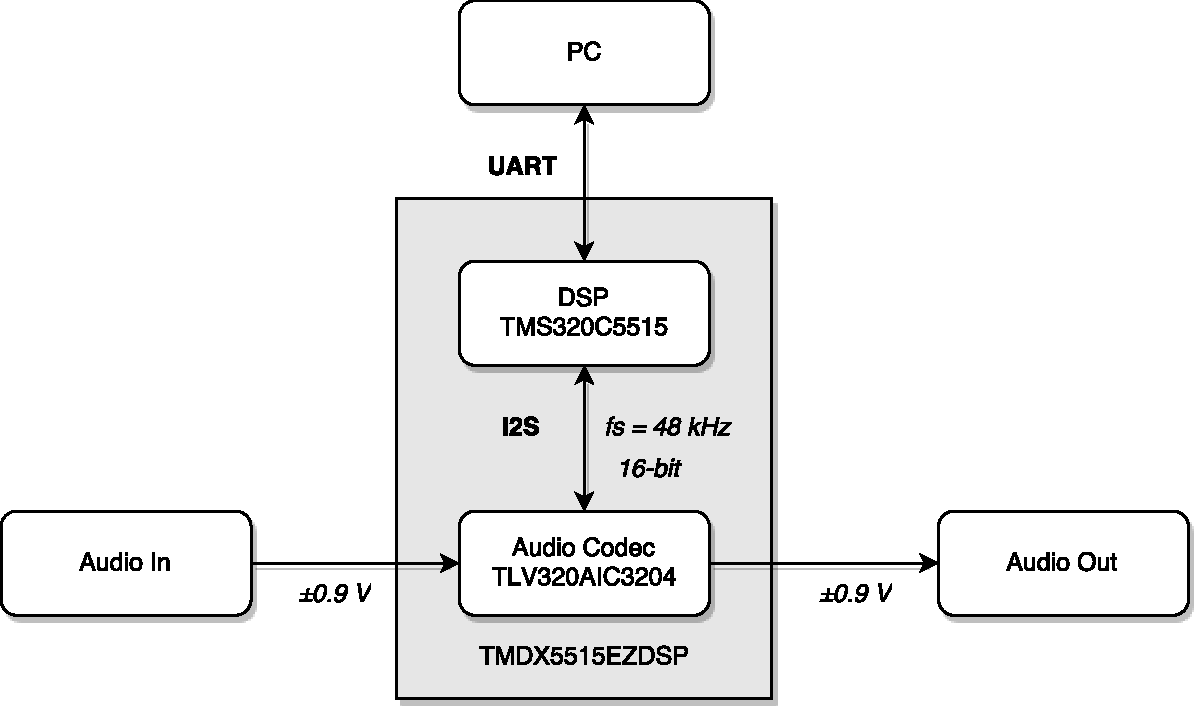
\includegraphics[width=0.75\textwidth]{figures/interfaceBlock.pdf}
\caption{}
\label{fig:interfaceBlock}
\end{figure}

\subsection*{I$^2$C Interface to Audio Codec}

As mentioned the the audio codec supports a sampling rate of 96 kHz and at least 44.1 kHz. The bit-resolution of the audio codec can also be adjusted to 24-bit and 32-bit. A $\text{I}^2$C-bus is linked between the DSP and the audio codec to setup the registers in the audio codec. In \autoref{fig:i2c_aic3204} the communication protocol between the $\text{I}^2$C communication between the dsp and audio codec is shown, where the DSP works as the master of the bus. Since the same $\text{I}^2$C-bus is used to interface with the OLED-display, the DSP must transmit a 7-bit to specify the address of the audio codec. Afterwards a byte is transmitted to specify the register address for the next data byte which is transmitted afterwards.

\begin{figure}[H]
\centering
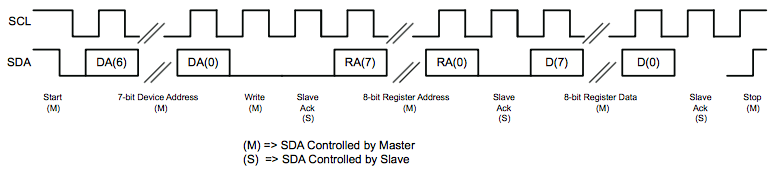
\includegraphics[width=0.98\textwidth]{i2c_aic3204}
\caption{Setup of the TLV320AIC3204 with $\text{I}^2$C.}
\label{fig:i2c_aic3204}
\end{figure}  

By using procedure above, the registers of the audio codec is then set to be mono, 16-bit and 48 kHz. When a audio sample is transmitted through the $\text{I}^2$S to the dsp, an interrupt flag for the $\text{I}^2$S is set high to tell the processor that data can be read from the data register. 

\subsection*{I$^2$S Audio Interface to Audio Codec}

To transfer audio data between the audio codec and DSP, a full-duplex Inter-IC Sound (I$"2$S)-bus is used. The I$"2$S-bus has a data a transmitter, receiver, clock, and frame synchronization. The transmitter and receiver is used for data exchange between the DSP and audio codec. The data transmitted consist of binary values thus the clock is used to synchronize the bit transmission between the DSP and audio codec. The frame synchronization bit can be seen as the sampling frequency, as the frame sync. transmits is set high.


\subsection*{Audio input and output}

The input and output of the audio codec are analog signals. According to the datasheet of the TLV320AIC3204 the audio codec the maximum input and output voltage are 0.5 $\text{V}_\text{RMS}$ or 0.7071 $\text{V}_\text{PEAK}$. If the input signal is above maximum voltage the audio codec will clip the signal. Therefore it must be ensured that the input voltage do not exceed 0.5 $\text{V}_\text{RMS}$. 

\subsection*{UART interface with PC}

To communicate with a PC, serial communication is used to exchange data between the DSP and PC. The development platform support UART interface through its expansion pins. Since UART is easy to implement, it has been chosen. Further more, the UART from the DSP needs to be converted to an USB protocol. To do so the RoHS TTL-232R-3V3-WE is used, as it has a chip that handles the conversion between USB and UART.









